\chapter{Desenvolvimento}\label{cap_desenv}

Para o desenvolvimento das atividades inicialmente foi escolhido duas base de dados. As bases foram encontradas no site http://cs.uef.fi/sipu/datasets/ onde possuem datasets próprios para a tarefa de clustering, os dataset não possuem informações de que se referem cada atributo ou cada instancia.

\section{Pré-processamento e Visualização}
Para realizar o pré-processamento foi necessário validar se os dados não possuiam números vazios ou algum tipo de valor que foge do esperado.


\section{Validação dos dados}
Foi validado que os dataset não possuem nenhum valor nulo ou valores diferentes de inteiro maior do que zero.

\section{Análise dos dados}
Com os valores todos normalizados podemos ver a correlação entre os atributos, que possuem alta relação em alguns casos. \ref{fig:correlacao}

\begin{figure}[h]
	\centering
	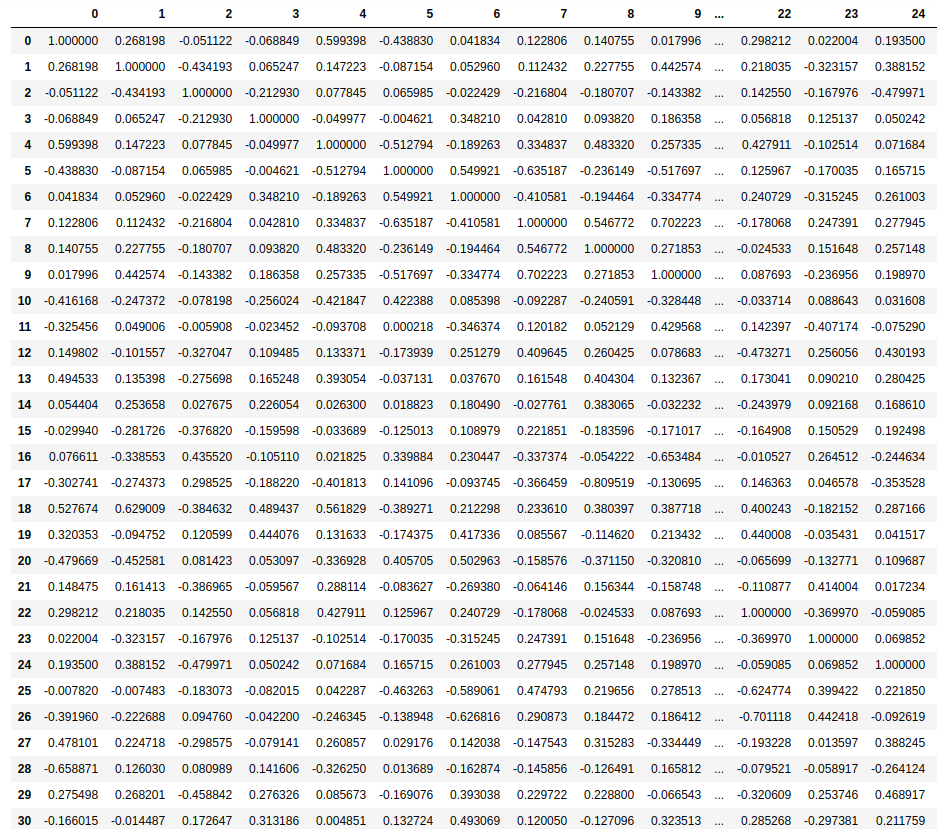
\includegraphics[width=0.7\linewidth]{images/corr}
	\caption{Correlação entre os dados.}
	Fonte: pessoal.
	\label{fig:correlacao}
\end{figure}

Após a visualazação dos dados foi gerado o bloxpot \ref{fig:bloxpot} para ver como está a distribuição dos dados onde é possível ver que poucos atributos possuem outliers e os dados possuem certa distribuição padrão, e também os valores de media, moda e mediana para cada atributo.\ref{fig:describe}

\begin{figure}[h]
	\centering
	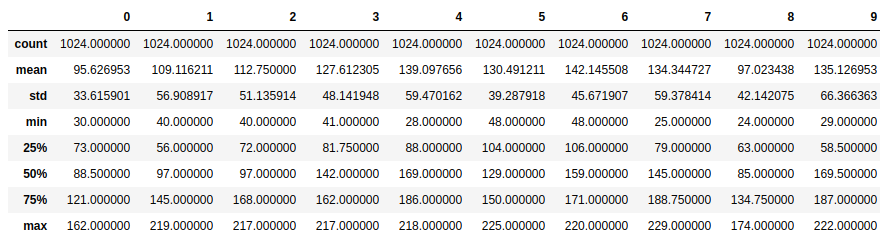
\includegraphics[width=0.7\linewidth]{images/describe}
	\caption{Distribuição dos dados.}
	Fonte: pessoal.
	\label{fig:describe}
\end{figure}

\begin{figure}[h]
	\centering
	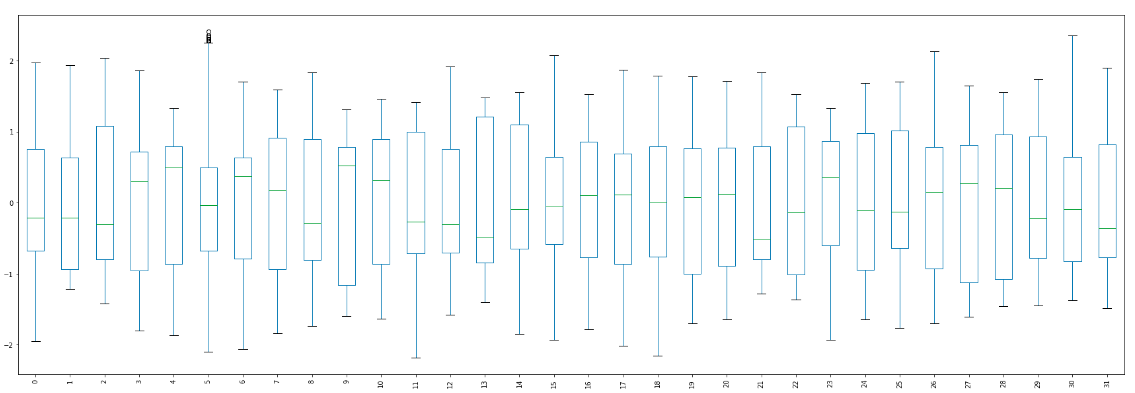
\includegraphics[width=0.7\linewidth]{images/bloxpot}
	\caption{Bloxpot exibindo outliers.}
	Fonte: pessoal.
	\label{fig:bloxpot}
\end{figure}


\section{Escalonamento}
Para aplicar os algoritmos de clustering, é necessário escalonar os dados, normalizando eles em uma faixa de -1 a 1, onde os dados irão manter a mesma proporção e similaridades.

\section{Algoritmos de Clustering}

Como solicitado na tarefa, deve ser aplicado 3 métodos de clustering  para visualização dos dados, o que foi selecionado neste caso são, K-means, Agglomerative Clustering
e por final Spectral Clustering.

Para todos os problemas foram selecionado 16 clusters, visto a quantidade de grupos, e de dados que possue o dataset.

Para execução dos algoritmos é utilizado a biblioteca sklearn, onde possui grande parte dos algoritmos de clustering já implementados

\section{Algoritmos de Clustering K-means dataset completo}

Como é possível visualizar abaixo, para o dataset completo o K-means gerou clusters bem esparços com centroides bem centralizados. \ref{fig:kmeansCompleto}

\begin{figure}[h]
	\centering
	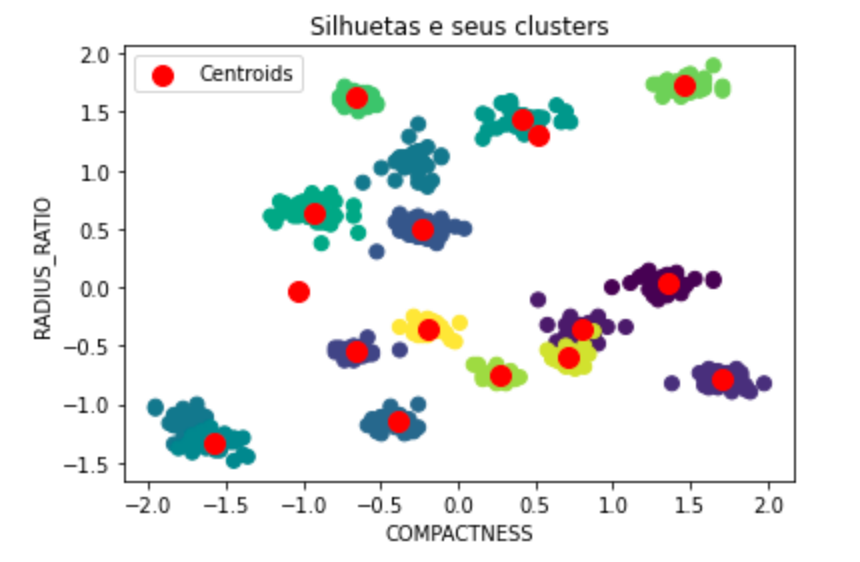
\includegraphics[width=0.7\linewidth]{images/kmeansCompleto}
	\caption{Algoritmo K-means com dataset completo.}
	Fonte: pessoal.
	\label{fig:kmeansCompleto}
\end{figure}

\section{Algoritmos de Clustering Agglomerative Clustering dataset completo}

Como é possível visualizar abaixo, para o dataset completo o Agglomerative Clustering gerou clusters onde alguns estão se sobrepondo e com dados entre dois clusters, outros estao bem separados. \ref{fig:aglomerativeClusteringCompleto}

\begin{figure}[h]
	\centering
	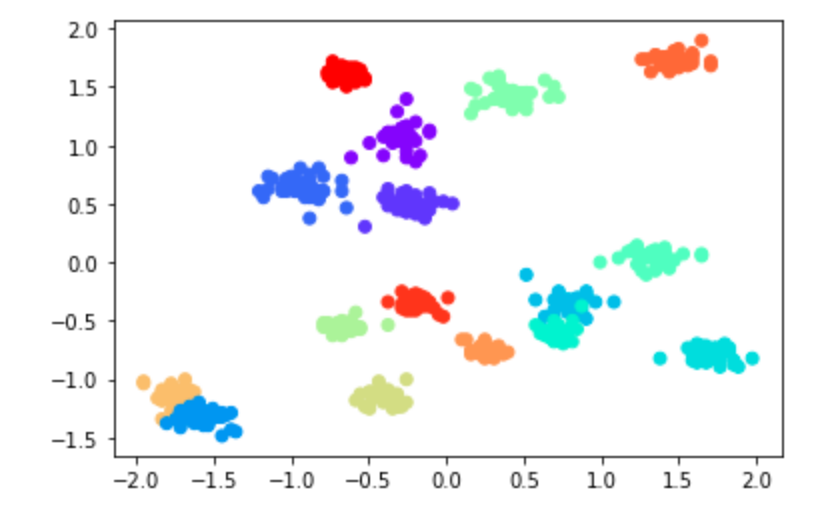
\includegraphics[width=0.7\linewidth]{images/aglomerativeClusteringCompleto}
	\caption{Algoritmo Agglomerative Clustering com dataset completo.}
	Fonte: pessoal.
	\label{fig:aglomerativeClusteringCompleto}
\end{figure}


\section{Algoritmos de Clustering Spectral Clustering dataset completo}

Como é possível visualizar abaixo, para o dataset completo o Spectral Clustering gerou alguns clusters que se sobrepoem e nem sempre estão bem esparcos. \ref{fig:spectralClusteringCompleto}

\begin{figure}[h]
	\centering
	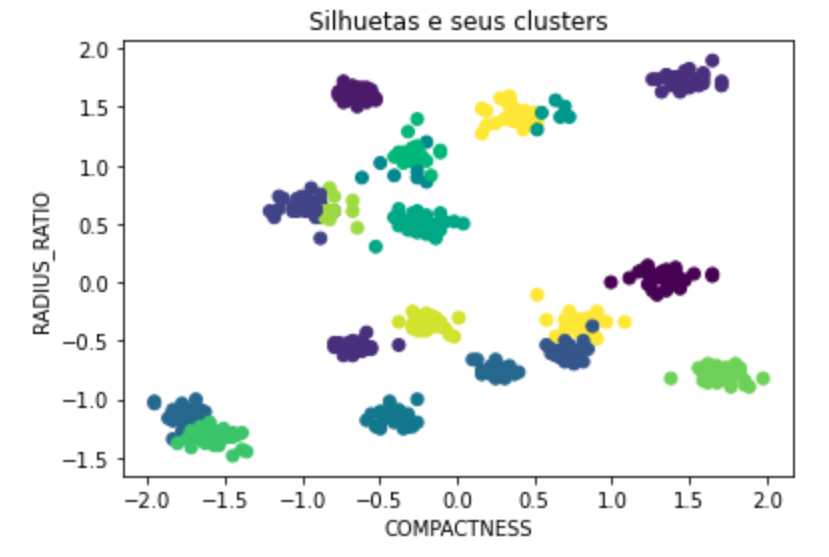
\includegraphics[width=0.7\linewidth]{images/spectralClusteringCompleto}
	\caption{Algoritmo Spectral Clustering com dataset completo.}
	Fonte: pessoal.
	\label{fig:spectralClusteringCompleto}
\end{figure}

\section{Seleção de atributos}

Após executar os três algoritmos de clustering com o dataset em questão, foi realizado um processo de seleção de atributos para realizar novamente a execução destes mesmos algoritmos.

O dataset possuia 32 atributos numericos, para realizar a selação foi utilizado um algoritmo que utiliza um parametro k como score para selecionar os melhores atributos.

Neste dataset o algoritmo selecionou apenas 4 atributos

\section{Algoritmos de Clustering K-means dataset selecionado}

Como é possível visualizar abaixo, para o dataset selecionado o K-means gerou clusters bem esparços com centroides bem centralizados. \ref{fig:kmeansSelecionado}

\begin{figure}[h]
	\centering
	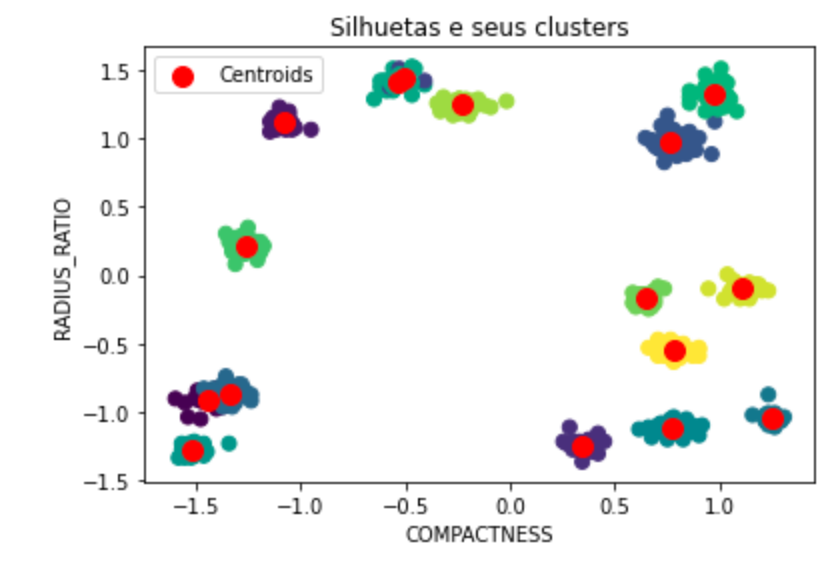
\includegraphics[width=0.7\linewidth]{images/kmeansSelecionado}
	\caption{Algoritmo K-means com dataset selecionado.}
	Fonte: pessoal.
	\label{fig:kmeansSelecionado}
\end{figure}

\section{Algoritmos de Clustering Agglomerative Clustering dataset selecionado}

Como é possível visualizar abaixo, para o dataset selecionado o Agglomerative Clustering gerou clusters onde alguns estão se sobrepondo e com dados entre dois clusters, outros estao bem separados. \ref{fig:aglometariveClusteringSelecionado}

\begin{figure}[h]
	\centering
	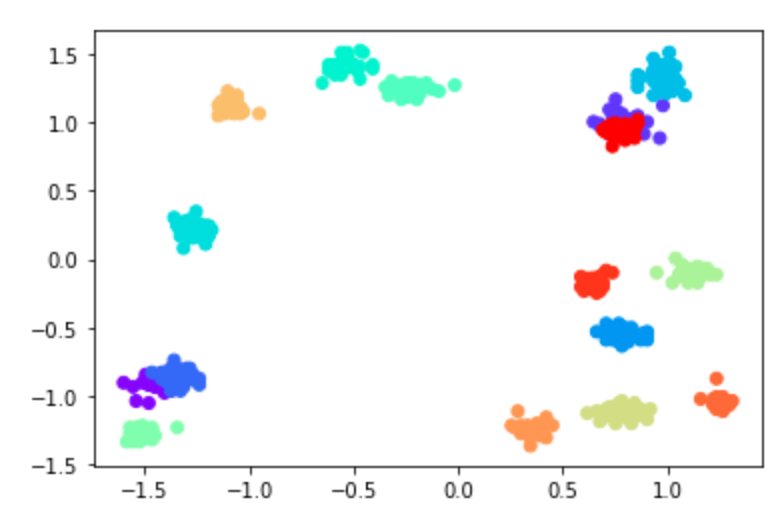
\includegraphics[width=0.7\linewidth]{images/aglometariveClusteringSelecionado}
	\caption{Algoritmo Agglomerative Clustering com dataset selecionado.}
	Fonte: pessoal.
	\label{fig:aglometariveClusteringSelecionado}
\end{figure}


\section{Algoritmos de Clustering Spectral Clustering dataset selecionado}

Como é possível visualizar abaixo, para o dataset selecionado o Spectral Clustering gerou alguns clusters que se sobrepoem e nem sempre estão bem esparcos. \ref{fig:spectralClusteringSelecionado}

\begin{figure}[h]
	\centering
	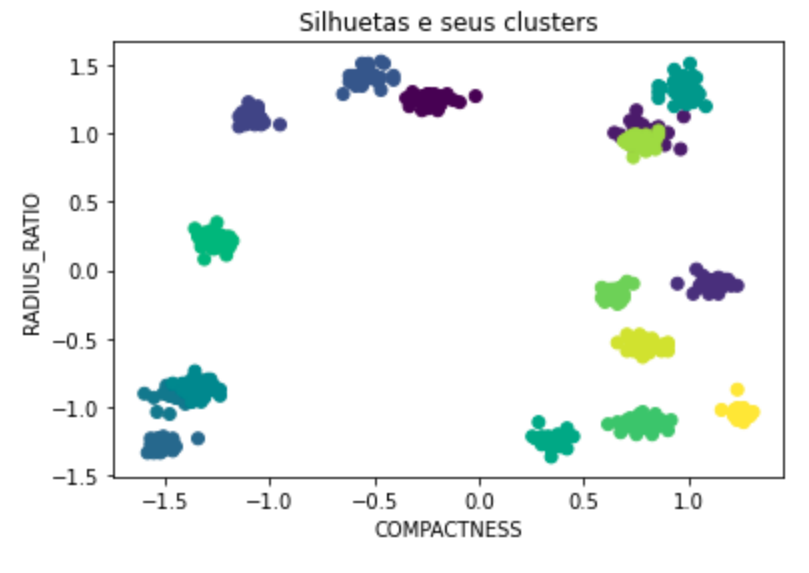
\includegraphics[width=0.7\linewidth]{images/spectralClusteringSelecionado}
	\caption{Algoritmo Spectral Clustering com dataset selecionado.}
	Fonte: pessoal.
	\label{fig:spectralClusteringSelecionado}
\end{figure}

\section{Análise de resultados}

Para analisar os resultados obtidos com os algoritmos foram utilizados 5 métodos de validação, dentre eles:

\begin{itemize}
	\item Confusion Matrix.
		
		Uma matrix exibindo todos os grupos gerados e seus erros e acertos, onde conta também os erros que devia ter colocado em uma categoria e deveria ser outra. (falsos positivos, falso negativo, verdadeiro positivo, verdadeiro negativo)

		Neste método, os valores na diagonal significam os valores que foram preditos corretamente, neste caso quanto mais numeros na diagonal mais o modelo acertou.
	
	\item Calinski-Harabaz Score
		
		Um indicativo que leva em conta dispersão interna do cluster e também a dispersão entre os clusters, um valor também entre -1 e 1 que quanto mais próximo de 1 melhor é seu resultado.
	
	\item Adjusted-Rand Score
	
		É um indicativo de validação interna do cluster onde o valor possível é entre -1 e 1 que valida quanto os pontos internos do cluster são similares, então quanto mais próximo de 1 melhor os clusters estão definidos.
	
	\item Adjusted Mutual Info Score
	
		É um indicativo de similaridade externa do clusters, neste caso quanto mais próximo de 0 menos similaridade eles possuem, é o esperado visto que cada cluster não deve possuir pontos em comum e devem ser distintos.
	
	\item F1 Score
	
		Um indicativo que utiliza a precissão e o recall do modelo para dizer se ele está errando muito, ou acertando, quanto mais próximo de 1 mais o modelo está correto.
	
	\item Accuracy Score
	
		A acurácia calcula quanto o modelo acertou baseado no total de instancias do dataset. Neste caso quanto mais próximo de 1 mais o modelo está acertando suas predições.
		
		
	\item Silhouette Score
	
		Um indicativo que também determina quão bem foram classificados os itens dos clusters, quanto maior o indice melhor os clusters foram separados.
\end{itemize}

\section{K-Means completo}

Como podemos ver na figura exibindo os resultados do K-Means completo, \ref{fig:resultKMeansCompleto} o modelo tendeu a errar para uma classe especifica onde a maioria dos resultados se concentraram em um unico cluster, também podemos perceber um rand score baixo de apenas vinte porcento, onde não é considerado um bom valor. Seu score F1 é apenas de 37 porcento e a acuracia de 50 porcento, onde não demonstrou grandes resultados.

\begin{figure}[h]
	\centering
	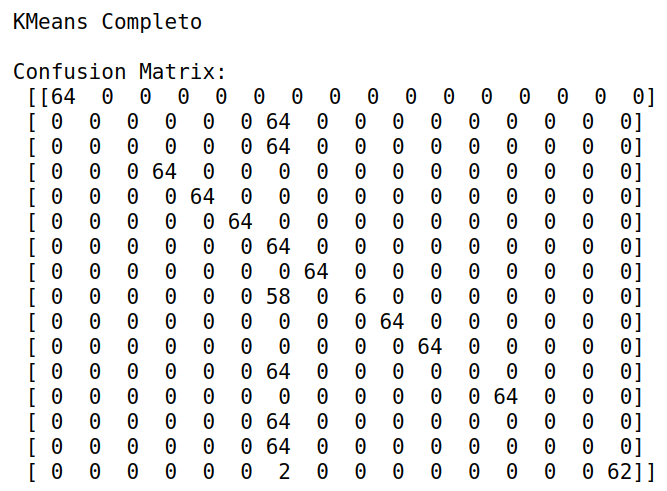
\includegraphics[width=0.7\linewidth]{images/resultKmeansCompleto}
	\caption{Métricas de validação do k-means}
	Fonte: pessoal.
	\label{fig:resultKMeansCompleto}
\end{figure}

\section{K-Means selecionado}

\begin{figure}[h]
	\centering
	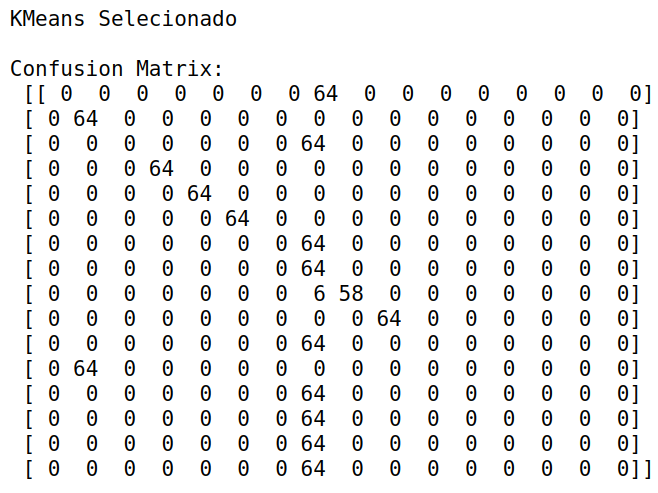
\includegraphics[width=0.7\linewidth]{images/resultKmeansSelecionado}
	\caption{Métricas de validação do k-means}
	Fonte: pessoal.
	\label{fig:resultKmeansSelecionado}
\end{figure}

\begin{figure}[h]
	\centering
	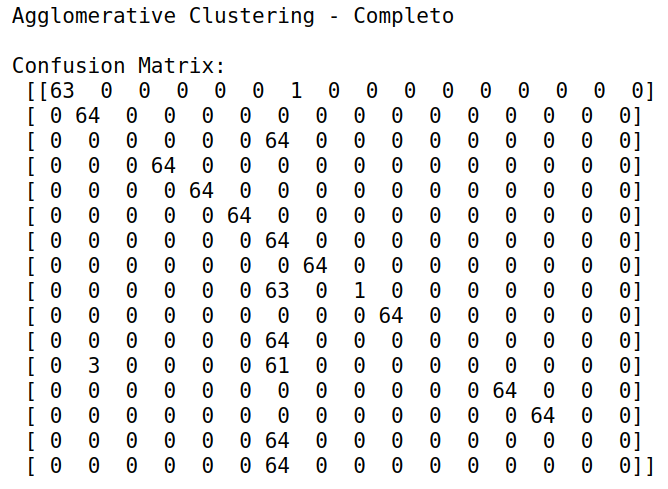
\includegraphics[width=0.7\linewidth]{images/resultsAglomerativeCompleto}
	\caption{Métricas de validação do k-means}
	Fonte: pessoal.
	\label{fig:resultAglomerativeCompleto}
\end{figure}

\begin{figure}[h]
	\centering
	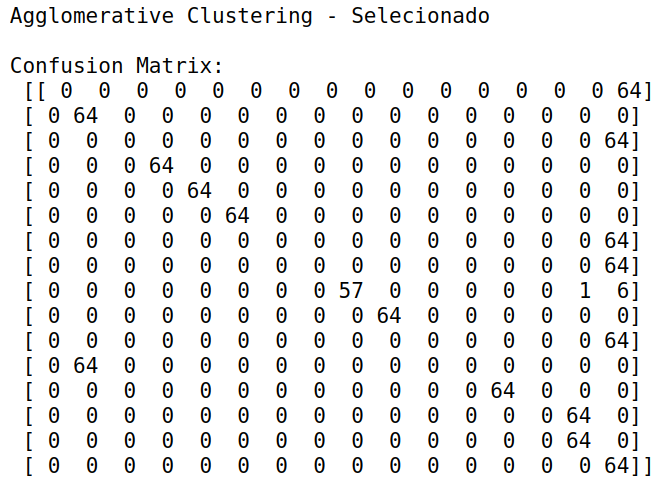
\includegraphics[width=0.7\linewidth]{images/resultsAglomerativeSelecionado}
	\caption{Métricas de validação do k-means}
	Fonte: pessoal.
	\label{fig:resultAglometariveSelecionado}
\end{figure}

\begin{figure}[h]
	\centering
	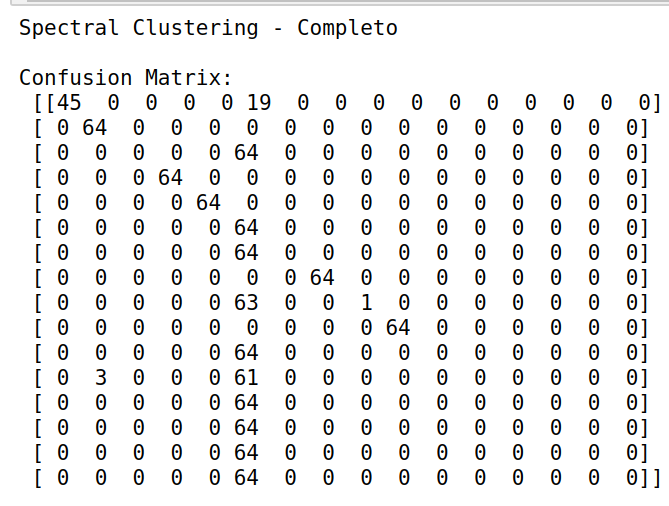
\includegraphics[width=0.7\linewidth]{images/resultSpectralCompleto}
	\caption{Métricas de validação do k-means}
	Fonte: pessoal.
	\label{fig:resultSpectralCompleto}
\end{figure}

\begin{figure}[h]
	\centering
	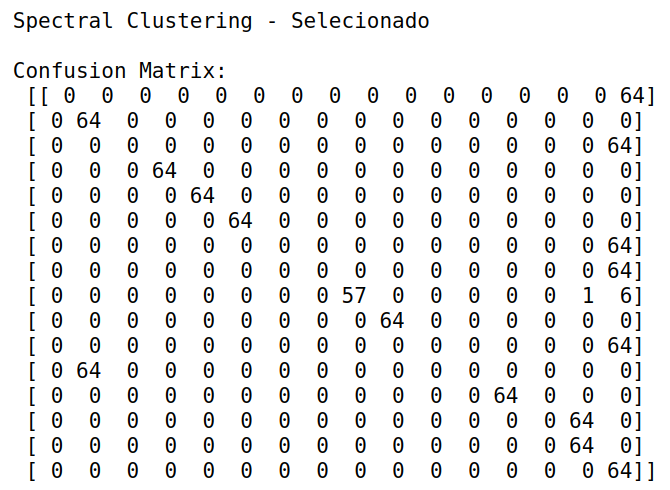
\includegraphics[width=0.7\linewidth]{images/resultSpectralSelecionado}
	\caption{Métricas de validação do k-means}
	Fonte: pessoal.
	\label{fig:resultSpectralSelecionado}
\end{figure}


\section{Segundo dataset}

Após realizar todos os experimentos com o dataset em questão, foi realizado um novo processamento com outro dataset, que possui mais dimensões, o código utilizado foi o mesmo, onde apenas foi alterado o arquivo de dados. Segue abaixo os resultados encontrados.


\section{Análise dos dados}

\begin{figure}[h]
	\centering
	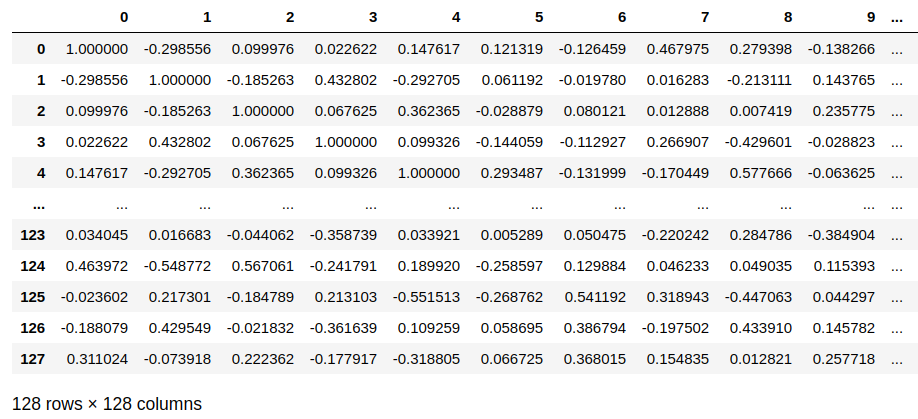
\includegraphics[width=0.7\linewidth]{images/dim128_corr}
	\caption{Correlação entre os dados.}
	Fonte: pessoal.
	\label{fig:dim128-correlacao}
\end{figure}


\begin{figure}[h]
	\centering
	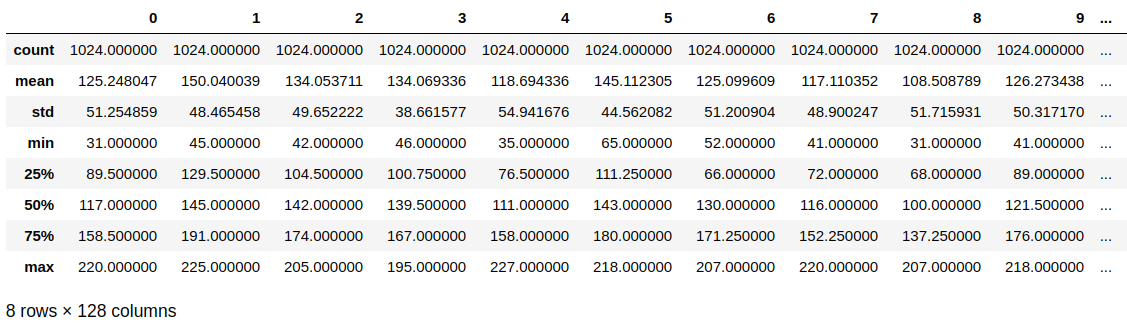
\includegraphics[width=0.7\linewidth]{images/dim128_describe}
	\caption{Distribuição dos dados.}
	Fonte: pessoal.
	\label{fig:dim128-describe}
\end{figure}

\begin{figure}[h]
	\centering
	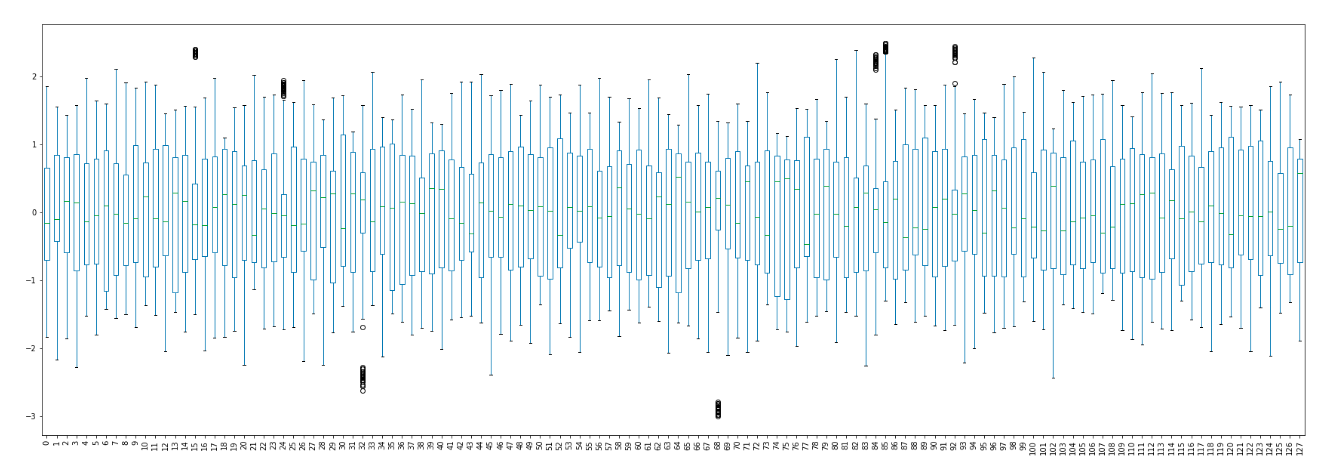
\includegraphics[width=0.7\linewidth]{images/dim128_bloxpot}
	\caption{Bloxpot exibindo outliers.}
	Fonte: pessoal.
	\label{fig:dim128-bloxpot}
\end{figure}


\section{Algoritmos de Clustering Completo}

\section{Algoritmos de Clustering K-means dataset completo}

Como é possível visualizar abaixo, para o dataset completo o K-means gerou clusters bem esparços com centroides bem centralizados. \ref{fig:dim128_kmeans_completo}

\begin{figure}[h]
	\centering
	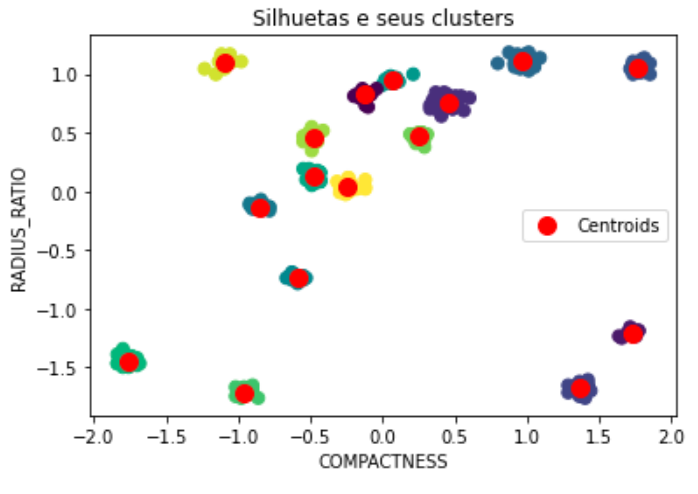
\includegraphics[width=0.7\linewidth]{images/dim128_kmeans_completo}
	\caption{Algoritmo K-means com dataset completo.}
	Fonte: pessoal.
	\label{fig:dim128_kmeans_completo}
\end{figure}

\section{Algoritmos de Clustering Agglomerative Clustering dataset completo}

Como é possível visualizar abaixo, para o dataset completo o Agglomerative Clustering gerou clusters onde alguns estão se sobrepondo e com dados entre dois clusters, outros estao bem separados. \ref{fig:dim128_agglomerative_completo}

\begin{figure}[h]
	\centering
	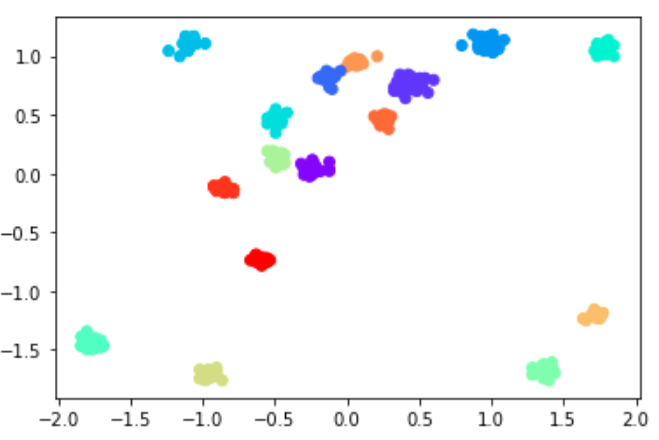
\includegraphics[width=0.7\linewidth]{images/dim128_agglomerative_completo}
	\caption{Algoritmo Agglomerative Clustering com dataset completo.}
	Fonte: pessoal.
	\label{fig:dim128_agglomerative_completo}
\end{figure}


\section{Algoritmos de Clustering Spectral Clustering dataset completo}

Como é possível visualizar abaixo, para o dataset completo o Spectral Clustering gerou alguns clusters que se sobrepoem e nem sempre estão bem esparcos. \ref{fig:spectralClusteringCompleto}

\begin{figure}[h]
	\centering
	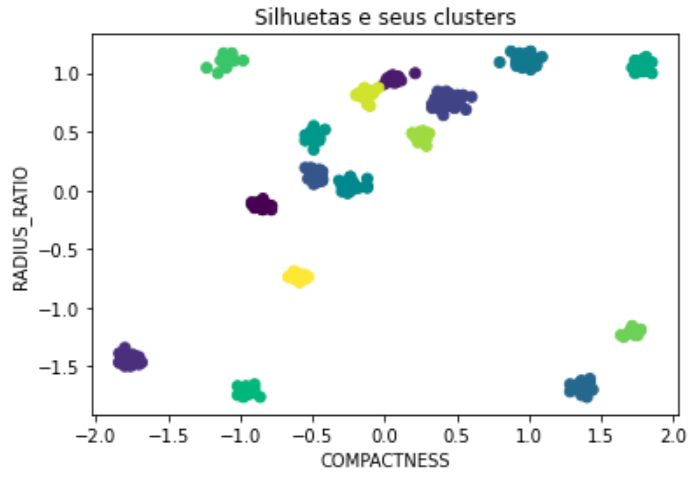
\includegraphics[width=0.7\linewidth]{images/dim128_spectral_completo}
	\caption{Algoritmo Spectral Clustering com dataset completo.}
	Fonte: pessoal.
	\label{fig:dim128_spectral_completo}
\end{figure}

\section{Algoritmos de Clustering Selecionado}

\section{Algoritmos de Clustering K-means dataset selecionado}

Como é possível visualizar abaixo, para o dataset selecionado o K-means gerou clusters bem esparços com centroides bem centralizados. \ref{fig:dim128_kmeans_selecionado}

\begin{figure}[h]
	\centering
	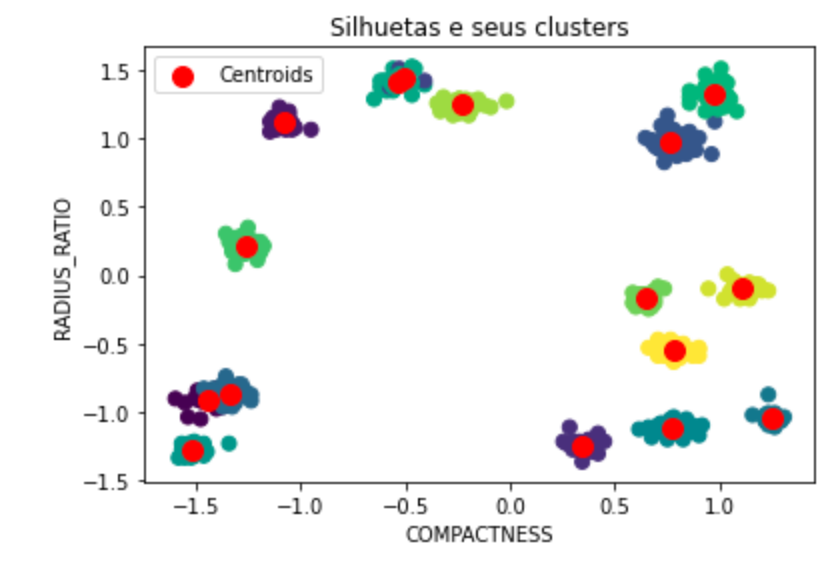
\includegraphics[width=0.7\linewidth]{images/kmeansSelecionado}
	\caption{Algoritmo K-means com dataset selecionado.}
	Fonte: pessoal.
	\label{fig:dim128_kmeans_selecionado}
\end{figure}

\section{Algoritmos de Clustering Agglomerative Clustering dataset selecionado}

Como é possível visualizar abaixo, para o dataset selecionado o Agglomerative Clustering gerou clusters onde alguns estão se sobrepondo e com dados entre dois clusters, outros estao bem separados. \ref{fig:dim128_agglomerative_selecionado}

\begin{figure}[h]
	\centering
	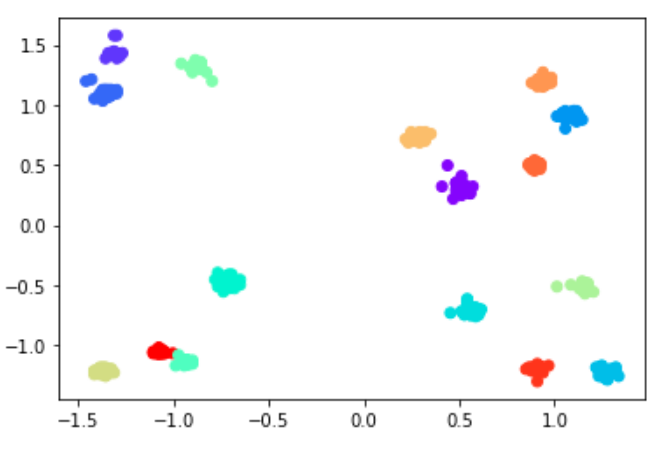
\includegraphics[width=0.7\linewidth]{images/dim128_agglomerative_selecionado}
	\caption{Algoritmo Agglomerative Clustering com dataset selecionado.}
	Fonte: pessoal.
	\label{fig:dim128_agglomerative_selecionado}
\end{figure}


\section{Algoritmos de Clustering Spectral Clustering dataset selecionado}

Como é possível visualizar abaixo, para o dataset selecionado o Spectral Clustering gerou alguns clusters que se sobrepoem e nem sempre estão bem esparcos. \ref{fig:dim128_spectral_selecionado}

\begin{figure}[h]
	\centering
	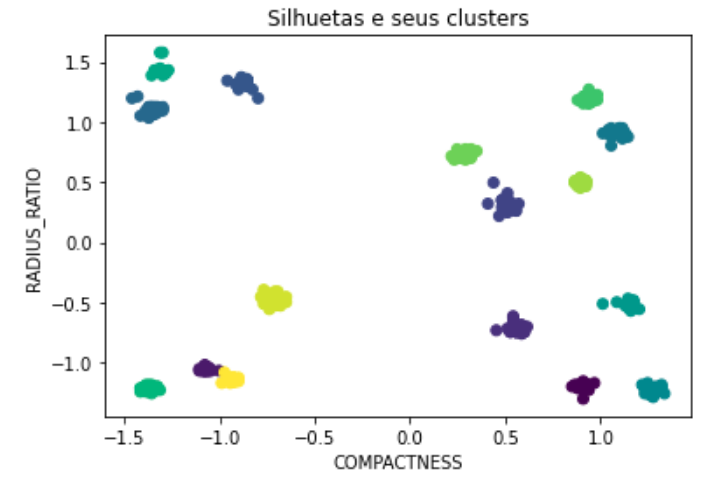
\includegraphics[width=0.7\linewidth]{images/dim128_spectral_selecionado}
	\caption{Algoritmo Spectral Clustering com dataset selecionado.}
	Fonte: pessoal.
	\label{fig:dim128_spectral_selecionado}
\end{figure}

\section{Análise de resultados}

\begin{figure}[h]
	\centering
	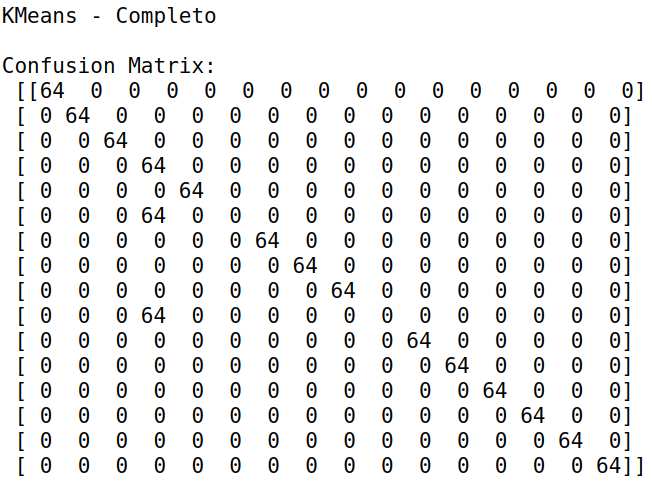
\includegraphics[width=0.7\linewidth]{images/dim128_result_kmeans_completo}
	\caption{Métricas de validação do k-means}
	Fonte: pessoal.
	\label{fig:dim128_result_kmeans_completo}
\end{figure}

\begin{figure}[h]
	\centering
	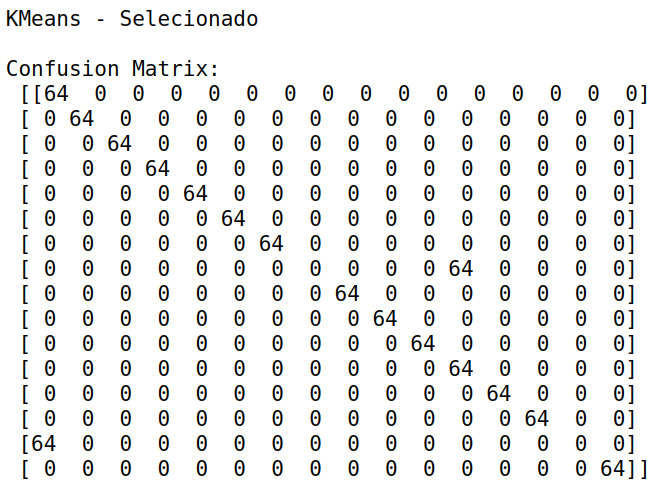
\includegraphics[width=0.7\linewidth]{images/dim128_result_kmeans_selecionado}
	\caption{Métricas de validação do k-means}
	Fonte: pessoal.
	\label{fig:dim128_result_kmeans_selecionado}
\end{figure}

\begin{figure}[h]
	\centering
	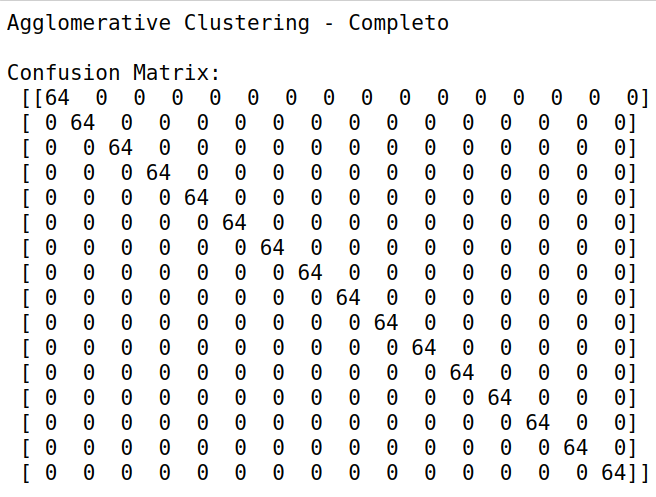
\includegraphics[width=0.7\linewidth]{images/dim128_result_agglomerative_completo}
	\caption{Métricas de validação do k-means}
	Fonte: pessoal.
	\label{fig:dim128_result_agglomerative_completo}
\end{figure}

\begin{figure}[h]
	\centering
	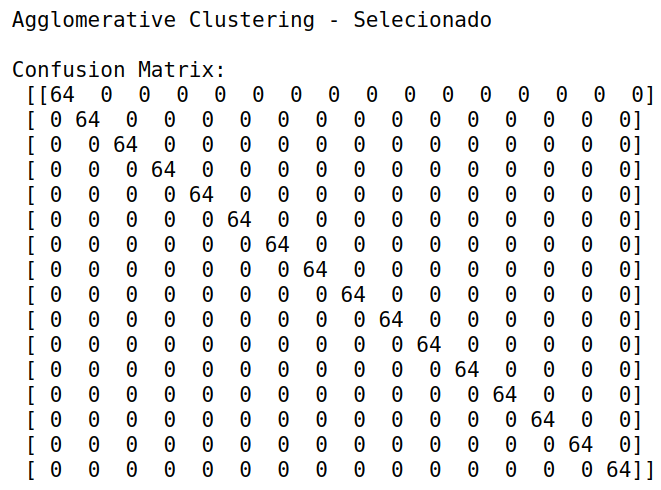
\includegraphics[width=0.7\linewidth]{images/dim128_result_agglomerative_selecionado}
	\caption{Métricas de validação do k-means}
	Fonte: pessoal.
	\label{fig:dim128_result_agglomerative_selecionado}
\end{figure}

\begin{figure}[h]
	\centering
	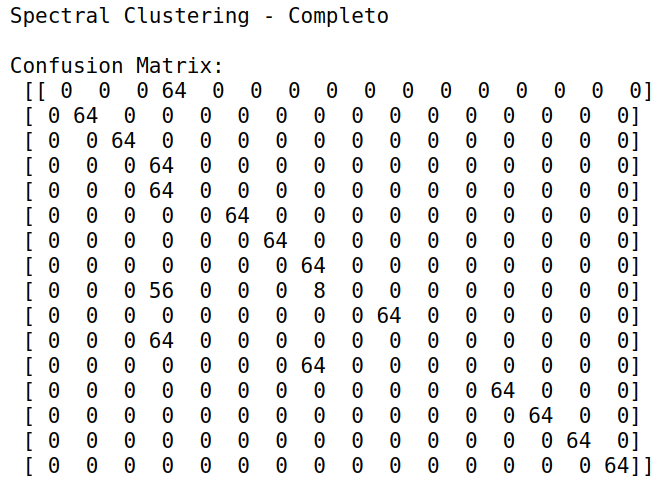
\includegraphics[width=0.7\linewidth]{images/dim128_result_spectral_completo}
	\caption{Métricas de validação do k-means}
	Fonte: pessoal.
	\label{fig:dim128_result_spectral_completo}
\end{figure}

\begin{figure}[h]
	\centering
	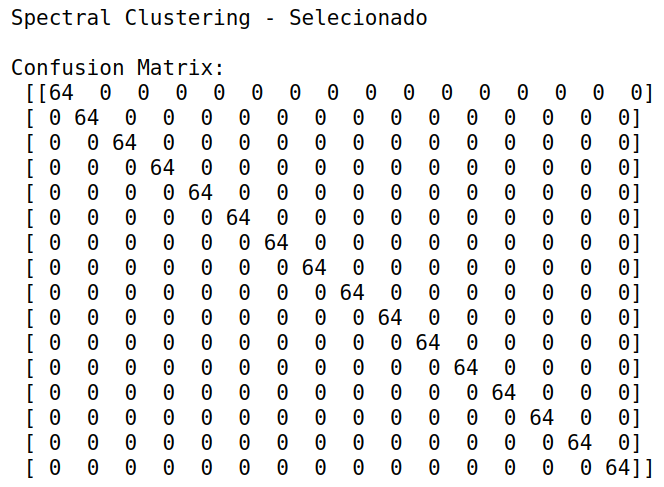
\includegraphics[width=0.7\linewidth]{images/dim128_result_spectral_selecionado}
	\caption{Métricas de validação do k-means}
	Fonte: pessoal.
	\label{fig:dim128_result_spectral_selecionado}
\end{figure}

\section{Resultados}

\section{Primeiro dataset}
A figura \ref{fig:resultDim032} representa os resultados obtidos com o primeiro dataset, onde é possível visualizar que houve uma melhora dos resultados obtidos com a redução do data set e também que 
o algoritmo de agglomerative com o dataset completo obteve melhor resultado.
\begin{figure}[h]
	\centering
	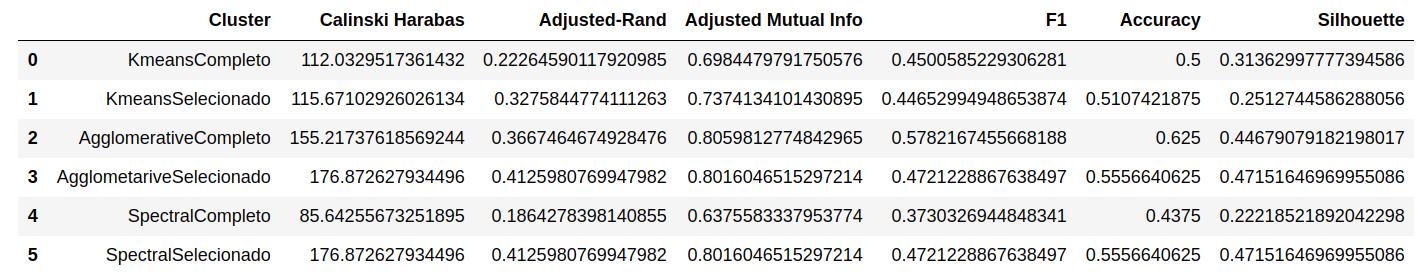
\includegraphics[width=0.7\linewidth]{images/result_dim032}
	\caption{Resultados para todos os clusters encontrados.}
	Fonte: pessoal.
	\label{fig:resultDim032}
\end{figure}

\section{Segundo dataset}
A figura \ref{fig:resultDim128} representa os resultados obtidos com o segundo dataset, onde é possível visualizar que houve uma melhora dos resultados obtidos com a redução do data set e também que 
alguns algoritmos conseguiram uma acuracia de 100%.
\begin{figure}[h]
	\centering
	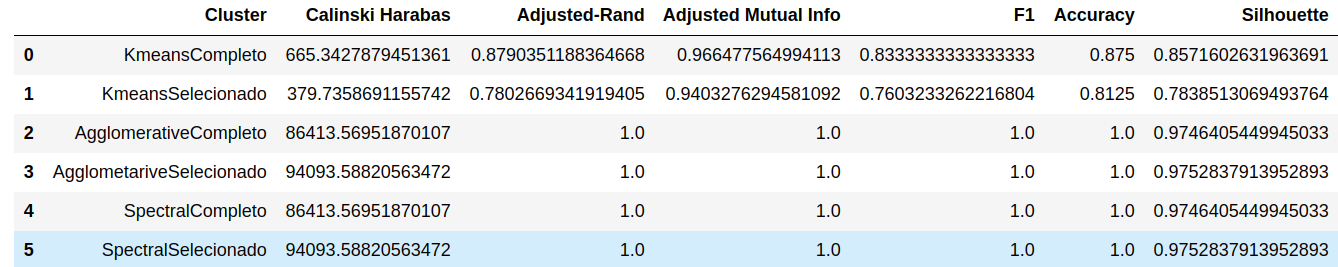
\includegraphics[width=0.7\linewidth]{images/result_dim128}
	\caption{Resultados para todos os clusters encontrados.}
	Fonte: pessoal.
	\label{fig:resultDim128}
\end{figure}